\begin{figure}[H]
  \centering
  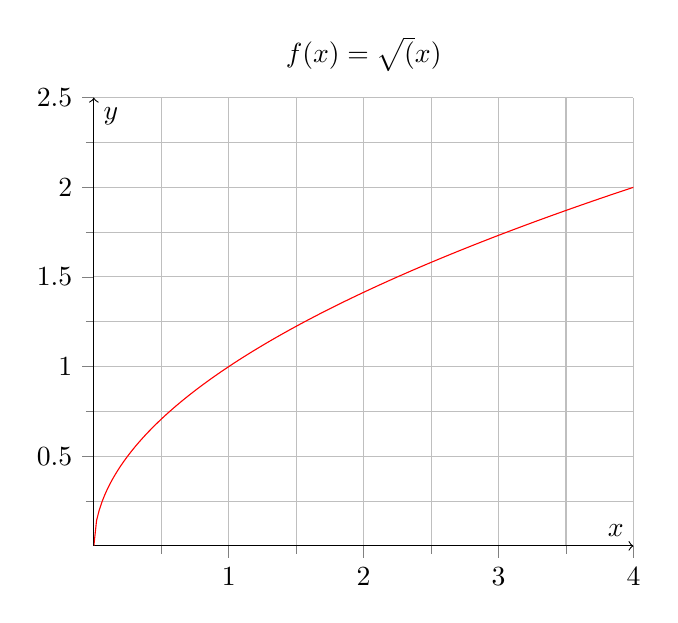
\begin{tikzpicture}
    \begin{axis}[
      xmin=0, xmax=4,
      ymin=0, ymax=2.5,
      axis x line=middle,
      axis y line=middle,
      axis line style={->},
      tick align=outside,
      grid=both,
      minor tick num=1,
      xlabel={$x$},
      ylabel={$y$},
      title={$f(x)=\sqrt(x)$}
    ]
      \addplot[ red, domain=0:4, samples=200] {sqrt(x)};
    \end{axis}
  \end{tikzpicture}
  \caption{Função afim $f(x)=\sqrt(x)$.}
\end{figure}